\newsection{Casi d'uso}
\subsection{Struttura}
Ogni caso d'uso è descritto dalla seguente struttura:
\begin{itemize}
	\item Codice identificativo: $$ \textbf{UC \{codice\_padre\}.\{codice\_figlio\}  } $$
	\begin{itemize}
		\item UC specifica che si tratta di un caso d'uso;
		\item Codice\_padre identifica univocamente i casi d'uso;
		\item Codice\_figlio è un numero progressivo che identifica i sottocasi.
	\end{itemize}
	\item Titolo;
	\item Diagramma UML;
	\item Attori;
	\item Scopo e descrizione;
	\item Precondizioni;
	\item Scenario principale;
	\item Postcondizioni;
	\item Inclusioni (se presenti);
	\item Estensioni (se presenti).
\end{itemize}
\Spazio
Inoltre il team ha individuato due casi d'uso generali (UCG1 e UCG2) la cui nomenclatura non segue quella appena riportata. Essi rappresentano i casi d'uso più ad alto livello, insieme anche ad UC5, con cui l'utente può interagire con il prodotto.
L'ambito d'azione del prodotto è distinguibile in due macro aree, una relativa alle operazioni che si possono effettuare sulla rete Bayesiana e l'altra relativa alle operazioni che comprendono la visualizzazione dei dati acquisiti.

\subsection{Attori}
L'attore che può interagire con il prodotto è soltanto uno:
\begin{itemize}
	\item \textbf{Utente}: si fa riferimento ad un utente generico, che ha intenzione di associare una rete Bayesiana ad un flusso dati per monitorare un'applicazione.
\end{itemize}

\newpage
\subsection{Caso d'uso generale UCG1: Operazioni sulla rete Bayesiana}
\begin{figure} [H]
	\centering
	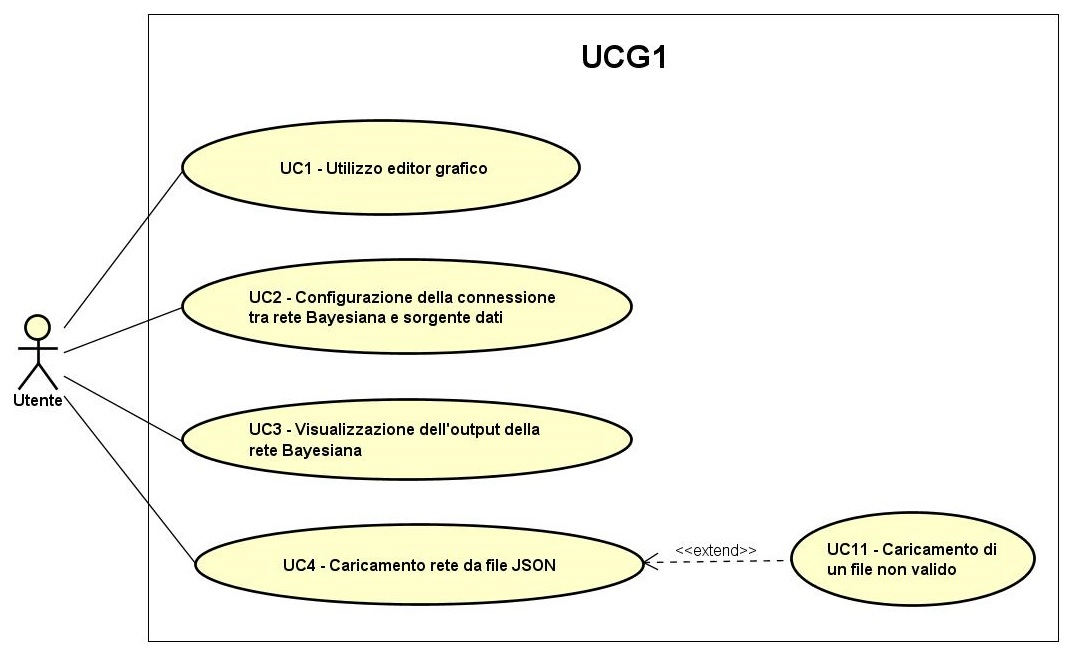
\includegraphics[scale=0.7]{Img/UCG1}
	\caption{UCG1 - Operazioni sulla rete Bayesiana}\label{}
\end{figure}
\begin{itemize}
	\item{\textbf{Attori primari}: Utente;}
	\item{\textbf{Scopo e descrizione}: l'attore vuole eseguire delle operazioni sulla rete Bayesiana;}
	\item{\textbf{Precondizione}: l'applicazione deve essere avviata correttamente e pronta all'uso;}
	\item{\textbf{Scenario principale}:
		\begin{itemize}
			\item{L'attore utilizza l'editor grafico (UC1);}
			\item{L'attore configura la connessione tra la rete e la sorgente dati (UC2);}
			\item{L'attore legge i dati acquisiti dalla rete Bayesiana (UC3)};
			\item{L'attore carica la definizione della rete da un file JSON (UC4).}
		\end{itemize}
	}
	\item{\textbf{Postcondizione}: l'attore ha eseguito le operazioni sulla rete Bayesiana.}
\end{itemize}

\subsection{Caso d'uso generale UCG2: Operazioni sulla visualizzazione dei dati}
\begin{figure} [H]
	\centering
	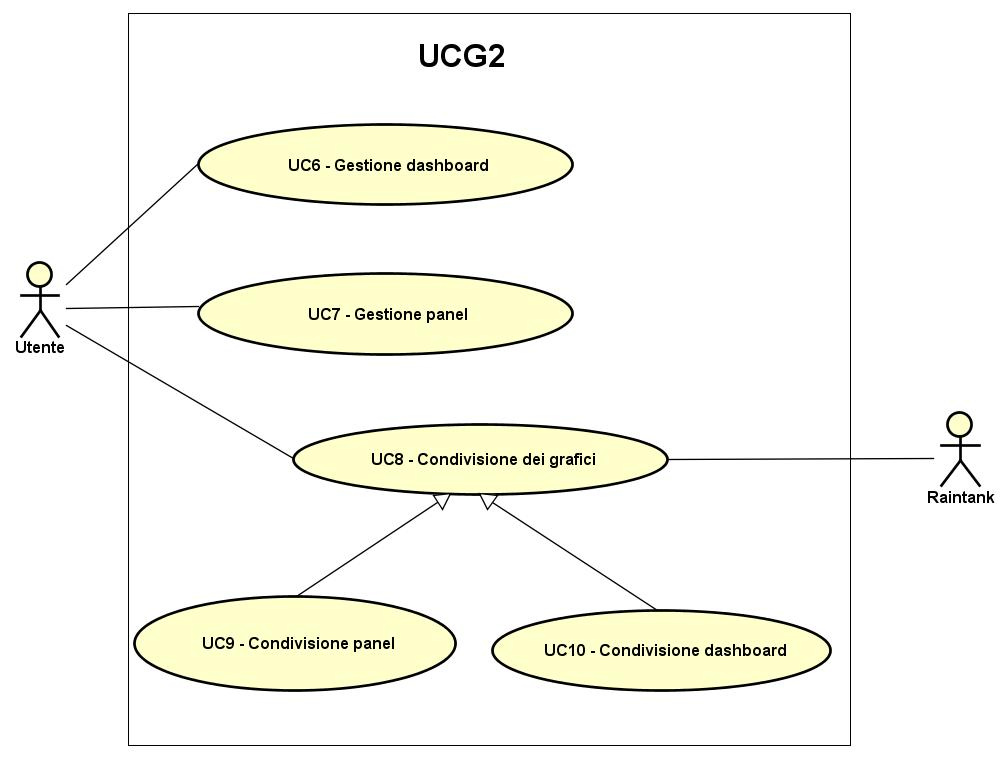
\includegraphics[scale=0.5]{Img/UCG2}
	\caption{UCG2 - Operazioni sulla visualizzazione dei dati}
\end{figure}
\begin{itemize}
	\item{\textbf{Attori primari}: Utente;}
	\item{\textbf{Scopo e descrizione}: l'attore vuole eseguire delle operazioni relative alla visualizzazione dei dati acquisiti;}
	\item{\textbf{Precondizione}: l'applicazione deve essere avviata correttamente ed in grado di leggere un flusso dati;}
	\item{\textbf{Scenario principale}:
		\begin{itemize}
			\item{L'attore modifica la struttura della dashboard (UC6);}
			\item{L'attore modifica la struttura di un panel (UC7);}
			\item{L'attore condivide i grafici ottenuti (UC8)}.
		\end{itemize}
	}
	\item{\textbf{Postcondizione}: l'attore ha eseguito le operazioni sulla visualizzazione dei dati.}
\end{itemize}
\newpage
